\documentclass[oneside,a4paper,english,links]{amca}
%
\usepackage{graphicx}
\usepackage{amsmath,amsfonts}

\title{INSTRUCTIONS TO PREPARE AN ARTICLE ACCORDING TO THE AMCA-STYLE}

\author[a,b]{First A. Author}
\author[b]{Second B. Author}
\author[b]{Third C. Author}
\author[a]{Fourth D. Author}
%
\affil[a]{Grupo de Mec\'anica Computacional,
Universidad Nacional de Villa Carolina,
Los Alerces 3492, 4200~Villa Carolina, Argentina,
gmc@uncarolina.edu.ar, \url{http://www.uncarolina.edu.ar/gmc}}
%
\affil[b]{Grupo de Ingenier\'\i{}a Aplicada,
Universidad Nacional de La Meseta,
Los Cipreses 3493, 4201~La Meseta, Argentina,
gia@unmeseta.edu.ar, \url{http://www.unmeseta.edu.ar/gia}}

%% NOTE: IF ALL AUTHORS BELONG TO THE SAME AFFILIATION
%% USE THE `\voidaffil' MACRO FOR THE AFFILIATION CODE.
%% Example:
%% \author[\voidaffil]{First A. Author}
%% \author[\voidaffil]{Second B. Author}
%% \author[\voidaffil]{Third C. Author}
%% \author[\voidaffil]{Fourth D. Author}
%% %
%% \affil[\voidaffil]{Grupo de Mec\'anica Computacional,
%% Universidad Nacional de Villa Carolina,
%% Los Alerces 3492, 4200 Villa Carolina, Argentina,
%% gmc@uncarolina.edu.ar, http://www.uncarolina.edu.ar/gmc}

\begin{document}
\vspace{3cm}

\maketitle

%% To set PDF METADATA: uncomment and replace fields in
%% UPPERCASE with appropriate values. 
%% 
%% \hypersetup{
%%   pdfauthor={AUTHORS},
%%   pdfkeywords={KEYWORDS},
%%   pdftitle={TITLE}
%% }
%%
%% For instance
%% \hypersetup{
%%   pdfauthor={Sponge B. and Star P.},
%%   pdfkeywords={multiphase flow, air-liquid mixtures},
%%   pdftitle={A new model for multi-phase flow}
%% }
%%
%% NOTE: To set the metadata is recommended but not absolutely
%% neccesary. 
%% This was done before with the \pdfinfo command,
%% but according to this post:
%% http://de.nntp2http.com/comp/text/tex/2008/12/5358fd061de9703a781885a5dcf98364.html
%% if `hyperref' is used, then you must use \hypersetup{} not \pdfinfo{}

\begin{keywords}
Instructions, AMCA style, Computational Mechanics, article.
\end{keywords}

\begin{abstract}
This document provides information and instructions for preparing an
article following the AMCA style. The first page is reserved for the
title of the article, the authors, affiliation, keywords and the
abstract. The abstract must be fully contained in the first page. The
Introduction must begin at the top of the second page. The first page
of the article will be printed in the book of abstracts. All the
instructions as well as the example files for \LaTeX{} and MS-Word can
be found in the web page of AMCA \url{http://www.amcaonline.org.ar}.
\end{abstract}

\section{INTRODUCTION}
This document provides information and instructions for preparing an
article according to the AMCA style. Only articles formatted according to
the present guidelines will be accepted for AMCA publications. 

\section{GENERAL SPECIFICATIONS}

The article may be written in English, Spanish or Portuguese within a
printing box of 16cm x 24cm, centered in the page. The paper including
figures, tables and references must have a minimum length of 4 pages
and must not exceed 25 pages. The paper must be uploaded to the AMCA
site in the form of a \textbf{PDF} file; no other formats (MS Word,
RTF) are accepted. The size of the PDF file of the paper must not
exceed 2~MBytes.

\subsection{Use of acronyms}

If acronyms are used, then define them before their first
occurrence. 

\section{TITLE, AUTHORS, AFFILIATION, KEYWORDS}

The first page must contain the Title, Author(s), Affiliation(s),
Keywords and the Abstract. The second page must begin with the
Introduction. The first line of the title is located 3cm from the top
of the printing box. 

\subsection{Title}

The title should be written centered, in 14pt, boldface Times Roman,
all capital letters. It should be single spaced if the title is more
than one line long. Inclusion of formulas or special characters in the
title is \textbf{highly} discouraged. Acronyms may be used if defined
\emph{in-line}, for instance ``Large Eddy Simulation (LES) of
flow around a cylinder''.

\subsection{Author}

The author's name should include first name, middle initial and last
name. It should be written centered, in 12pt boldface Times Roman,
12pt below the title. Put all the authors together, split in several
lines if necessary. Affiliations must be arranged in centered blocks,
after the authors. Identify each author with its corresponding
affiliation using a letter superscript, as in the example. If all the
authors belong to the same affiliation do not use superscript. 

\subsection{Affiliation}

Author's affiliation should be written centered, in 11pt Italic Times Roman,
12pt below the list of authors. A 12pt space should separate two
different affiliations. It is recommended that authors include an
e-mail address and a web page per affiliation site, if possible. 

\subsection{Keywords}

Please, write no more than six keywords.  They should be written left
aligned, in 12pt Times Roman, and the line must begin with the words
{\bf Keywords} boldfaced (use {\bf Palabras Clave} in Spanish and {\bf
Palavras Chave} in Portuguese). A 12pt space should separate the
keywords from the affiliations.

\subsection{Abstract}

Use 11pt Times Roman for the abstract. The word {\bf Abstract} must be
set in boldface, not italicized, at the beginning of the first line
(use {\bf Resumen} for Spanish and {\bf Resumo} for Portuguese). The
abstract text should be justified and separated 12pt from the
keywords, as shown in the first page of these instructions. The
abstract should be self-contained, so do not include figures, tables
or equations in the abstract. Neither include any reference to such
material. It is discouraged to include references to other work in the
abstract. In case of including any references, then they should be
included \emph{in-line} but abbreviated, as in this example (C. Jhonson
et.al., \emph{Int J Num Meth Eng}, 34(3):543--568 (1992); D. Mitchell and
J. Brady, \emph{J Sound Vib}, 21(2):221--230 (2006)). Multiple citations
should be separated by semi-colons. \textbf{It is strongly discouraged
to include more than 2 references in the abstract}. Inclusion of
formulas is \textbf{highly} discouraged. Avoid special
characters. If acronyms are used, then define them before their first
occurrence. 

\section{HEADINGS}

\subsection{Main headings}

The main headings should be written left aligned, in 12pt, boldface
and all capital Times Roman letters. There should be a 12pt space
before, and 6pt after the main headings.

\subsection{Secondary headings}

The secondary headings should be written left aligned, in 12pt,
boldface Times Roman, with an initial capital for first word only. There
should be a 12pt space before, and 6pt after the secondary headings.

\section{TEXT}

The normal text should be written single-spaced, justified, using 12pt
Times Roman in one column. The first line of each paragraph must be
indented 0.5cm. There is not inter-paragraph spacing.

\section{PAGE NUMBERS}

The authors {\bf must not number} the pages of the article. Numbers will
be added by the editor/publisher. 

\section{FIGURES}

All figures should be numbered consecutively and captioned. The
caption should be written centered, in 10pt Times Roman, upper and lower
case letters.

\begin{figure*}[htb]
\centerline{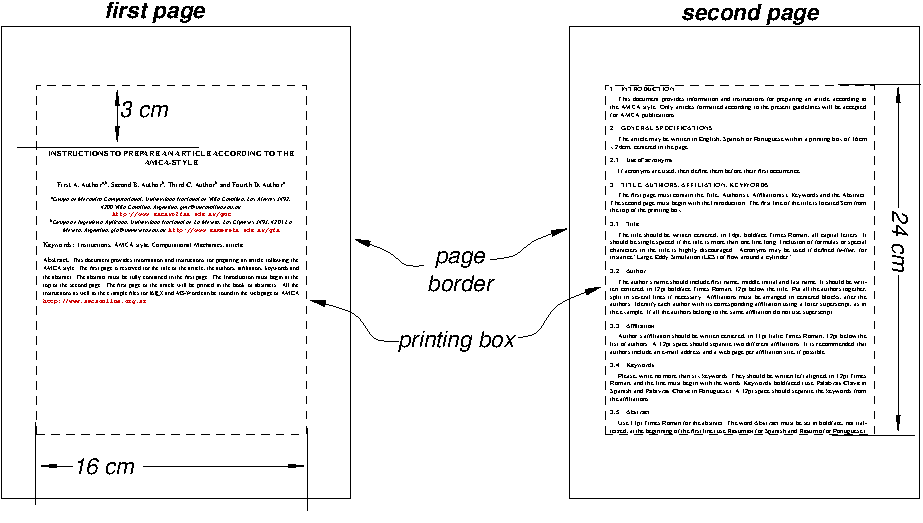
\includegraphics{firstpage}}
\caption{Page layout}
\label{fg:figure}
\end{figure*}

A 6pt space should separate the figure from the caption, and a
12pt space should separate the upper part of the figure and the
bottom of the caption from the surrounding text (see
Fig.~\ref{fg:figure}).

Figures should be referenced in the text. Color figures are welcomed.

\section{EQUATIONS}

A displayed equation is numbered, using Arabic numbers in parentheses.
It should be  centered, leaving a 6pt space above and below to separate it from
the surrounding text.

The following example is a simple single line
equation
%
\begin{equation}
Ax = b.
\end{equation}

The next example is a multi-line equation
%
\begin{equation} \label{eq:simple}  
\begin{aligned}
Ax& = b,\\
Ax& = c.
\end{aligned}
\end{equation}
%
If possible, internal PDF links must be generated for references to
equations. The recommended color for links to references in the text
is blue (e.g., see Eq.~(\ref{eq:simple})).

\section{TABLES}

All tables should be numbered consecutively and captioned, the caption
should be 10pt Times Roman, upper and lower case letters.

A space of 6pt separates the table from the caption, and 12pt space
separates the table from the surrounding text. For an example, see
Table~\ref{tab:n50}. Tables should be referenced in the text.

\begin{table}[htb]
\centering
\begin{tabular}{|c|c|c|c|}
\hline  & 20x20 mesh & 50x50 mesh & 100x100 mesh\\
\hline
\hline
 0 & 41.00 & 1.00 & 4.92\\
\hline
 1 & 40.86 & 1.02 & 4.88 \\
\hline
10 & 23.81 & 3.44 & 2.92 \\
\hline
50 & 5.62 & 64.20 & 1.08 \\
\hline
\end{tabular}
\caption{Condition number for the Stekhlov operator. }
\label{tab:n50}
\end{table}

\section{FORMAT OF REFERENCES}

References should be quoted in the text using the \emph{author-style}
(a.k.a. \emph{Harvard style}). References can be cited in
\emph{parenthetical} form \citep{zienkiewicz91,idelsohn94,meyer82,meyer82b}, or
in \emph{textual} form, e.g. see
\citet{zienkiewicz91,idelsohn94,meyer82,meyer82b}.  References are grouped
together and sorted alphabetically at the end of the article as shown
in these instructions. Do not include references that are not cited in
the article body. 

If possible, internal PDF links must be generated for citations. The
recommended color for links to references in the text is blue. The
preferred color for links to external references, as web pages, 
is red (e.g. \url{http://www.amcaonline.org.ar}).

\section{CONCLUSIONS}

Template files in TeX, \LaTeX{} and MS-Word may be found at the
AMCA web site: \url{http://www.amcaonline.org.ar}. 
Remember: {\bf Do not number the pages.}
%
\bibliography{amcapaper}
\end{document}
% $Id: amcapaper.tex,v 1.23 2006/08/14 16:58:45 mstorti Exp $
